\documentclass[12pt,a4paper,oneside]{report}
\usepackage[utf8]{inputenc}
\usepackage[english]{babel}
\usepackage{amsmath}
\usepackage{amsfonts}
\usepackage{amssymb}
\usepackage{graphicx}
\usepackage[left=2cm,right=2cm,top=2cm,bottom=2cm]{geometry}
\author{Daniel Aguiar da Silva Carvalho}
\begin{document}
\sffamily
\begin{center}
\textbf{\large{Thesis Advancement Report 2014-2015 (First Year)}}
\end{center}

\begin{flushleft}
\textbf{Thesis title:} Trusted-SLA Guided on Multi-cloud Environments \\
\textbf{PhD. student:} Daniel Aguiar da Silva Carvalho \\
\textbf{Supervisor:} Chirine Ghedira-Guegan \\ 
\textbf{Co-supervisors:} Nadia Benani and Genoveva Vargas-Solar
\end{flushleft}


\begin{flushleft}
\textbf{1 Context}\\
\end{flushleft} 

The data integration is a well-known and widely studied problem in the database area. 
It consists in merging data from different data sources and granting a unified view of the data~\cite{Lenzerini:2002}. 
%
In this area, the contributions can be divided in: (i) providing a global integrated representation of different data collections. This can be done either by defining a schema (e.g., global and local as view approaches), by tagging data with meta-data or by associating them to knowledge (e.g. semantic Web approaches); and (ii) The integration and the deployment architectures used for integrating data (i.e. Cloud, federated databases, etc).
%
Cloud computing opens new challenges to data integration. 
The possibility of an unlimited access to resources that arises changes the way to process data.
In this context, some data integration approaches have been proposed.
\cite{Gonzalez:2010b} proposed a cloud-based data management and integration system.
It enables data sharing, integration and collaboration between multiple users according to some design foundations (such as integration in the Web, incentives for sharing and facilitate collaboration). 
%It enables data sharing, integration and collaboration between multiple users. 
%According to some design foundations (such as integration in the Web, incentives for sharing and facilitate collaboration), the authors described the system  and some examples of applications that can take advantages from it. 
\cite{Gonzalez:2010} described in detail the system architecture, integration process, query processing proposed by~\cite{Gonzalez:2010b}. 
%Additionally, an API and an example of an integrated application with Google Maps is presented. 
\cite{078} combined data integration, service oriented architecture and distributed processing. 
The Service Oriented Data Integration based on MapReduce System (SODIM) works on a pool of collaborative services and can process a large number of databases represented as web services. 

%The data integration is a well-known and widely discussed problem in the database area. It consists in merging data from different data sources and granting a unified view of the data~\cite{Lenzerini:2002}. 
%
%Considering this, cloud and multi-cloud computing opens new challenges to data integration. 
%The possibility of an unlimited access to resources that arises with the cloud model changes the way to process data.
%In this context, some data integration approaches have been proposed.
%\cite{Gonzalez:2010b} proposed a cloud-based data management and integration system.
%It enables data sharing, integration and collaboration between multiple users. 

%According to some design foundations, such as integration with the web, easy of use, incentives for sharing and facilitate collaboration, the authors described the system  and some examples of applications that can take advantages from it. 

%\cite{Gonzalez:2010} described in detail the system architecture, integration process, query processing proposed by~\cite{Gonzalez:2010b}. 
%Additionally, an API and an example of an integrated application with Google Maps is presented. 
%\cite{078} combined data integration, service oriented architecture and distributed processing. 
%The Service Oriented Data Integration based on MapReduce System (SODIM) works on a pool of collaborative services and can process a large number of databases represented as web services. 
%
%In the cloud scenario, it is a hard task to one single cloud deliver the resources necessaries to fit customer requirements. 
%To avoid this, cloud providers began to share their computing resources.
%This new (multi)-cloud configuration add more challenges to data integration, considering the large amount and diversity of data, and quality and security aspects of the integration.
%The data privacy is the most tackled aspect in this context.

In the cloud scenario, one cloud cannot be expected to provide the necessary resources to fulfill application requirements. 
%In the cloud scenario, it is a hard task to one single cloud deliver the resources necessaries to fit customer requirements. 
%To avoid this, cloud providers began to share their computing resources.
Therefore, applications have started to address different cloud providers for externalizing different data processing and management resources.
This new (multi)-cloud configuration add more challenges to data integration, considering the large amount and diversity of data, and quality and security aspects of the integration.
Data privacy is the most popular aspect in this context.
\cite{YauY08} proposed a privacy-preserving repository in order to integrate data. 
Based on users' integration requirements, the repository supports the retrieval and integration of data across different services. 
\cite{096} introduced an inter-cloud data integration system that considers a trade-off between users' privacy requirements and the cost for protecting and processing data.
%According to the users' privacy requirements, the query plan in the cloud repository 
%creates the users' query. 
%This query is subdivided into sub-queries that can be executed in  service providers or on a cloud repository.
%Each option has its own  privacy and processing costs.
%Thus, the query plan executor decides the best location to execute the sub-query
%to meet privacy and cost constraints. 
To be synthesized, other quality aspects of data integration services have been highlighted in~\cite{Dustdar:2012}.

\bigskip
In cloud computing, a common way of defining requirements and obligations between the \textit{cloud provider} and \textit{cloud customer} is through service level agreement (SLA). 
SLAs have been widely adopted in the cloud context. 
\cite{011} presented a approach for security service level agreements on hybrid clouds focussing on the lifecycle of a security SLA, considering some security mechanisms (i.e. secure resource pooling, secure elasticity, access control, audit, verification and compliance, and incident management and response).
\cite{009} introduced a generic SLA model that includes management capabilities as a service which are agreed and negotiated in contracts. 
These management capabilities (elasticity, high availability, scalability and on demand provisioning) are performed by managing services called Pcloud services. 
The idea is to help the cloud customer to choose the appropriated providers that fits his requirements. 
\cite{005} designs SLA based on functional and non-functional requirements of the different cloud delivery models.

Summarizing, the contributions can be divided in two groups: (i) approaches focussing on the SLA negotiation phase; and (ii) approaches for monitoring and allocation of resources  to detect and avoid SLA violations. Among them, we identified one single approach regarding data integration in a grid environment guided by SLA~\cite{Nie07}.
%We believe that data integration can take advantages by integrating SLA on its solutions. 
%To the best of our knowledge, we have not identified any other proposal adopting the use of SLAs combined with a data integration approach on a (multi)-cloud context.

%In cloud computing, a common way of defining requirements and obligations between the \textit{cloud provider} and \textit{cloud customer} is through service level agreement (SLA) contracts. 
%SLAs have been widely adopted in the cloud context. 
%
%\cite{011} presented a approach for security service level agreements on hybrid clouds. The author focus on the lifecycle of a security SLA, considering some security mechanisms (i.e. secure resource pooling, secure elasticity, access control, audit, verification and compliance, and incident management and response).
%
%\cite{009} introduced a generic SLA model that includes management capabilities as a service which are agreed and negotiated in contracts. These management capabilities (elasticity, high availability, scalability and on demand provisioning) are performed by management services called Pcloud services that are defined in order to achieve application requirements. The idea is to help cloud customer to choose the appropriated providers that fits his requirements. 
%
%\cite{005} focused on the designing step of the SLA. 
%Based on functional and non-functional requirements of the different cloud delivery models, a conceptual framework for cloud computing is proposed. 
%The objective is to enhance trust and reliability between the parts in the negotiation phase.

%Summarizing, the contributions are divided in two groups: (i) approaches focus on the SLA negotiation phase; and (ii) approaches for monitoring and allocation of resources in order to detect and avoid SLA violations. Among them, we identified one single approach regarding data integration in a grid environment guided by SLA~\cite{Nie07}.

We believe that data integration on multi-cloud environments can take advantage by integrating SLA on its solutions. To the best of our knowledge, we have not identified any other proposal adopting the use of SLAs combined with a data integration approach on a (multi)-cloud context.

\begin{flushleft}
\textbf{2 Problem Statement}\\
\end{flushleft}

We assume that data integration is done on a (multi)-cloud service oriented environment. We also consider that data integration is done under new conditions with respect to the type of data sources, the environment where it is performed and the preferences  of data consumers and the SLA. 
SLA measures can be monitored in all cloud providers and negotiated. Data are provided as services that export APIs to retrieve data and processing methods. 
We suppose that cloud services and data services are listed in a registry.

Let us show an example from the domain of energy management to illustrate our problem. 
For instance, we assume we are interested in queries expressed in an SQL-like language associated to a set of QoS preferences expressing the requirements of the user like: \textit{Give a list of energy providers that can provision 1000 KW-h, in the next 10 seconds, that are close to my city, with a cost of 0,50 Euro/KW-h and that are labeled as green?} The problem here is how can the user efficiently obtain results for her queries, meeting her QoS requirements, respecting her subscribed contracts with the involved cloud provider(s), and without neglecting services contracts? 
Particularly, for queries that call several services deployed on different clouds.

%In our vision a query expressed in an SQL-like language is associated to a set of QoS preferences expressing the requirements of the user. For example, the economic cost she is ready to pay for executing the query, the provenance of the data, the reputation of data services and the expected time response. The answer of such a query is the result of integrating data from different services according to a series of phases described in the following section.

\begin{flushleft}
\textbf{3 Objectives}\\
\end{flushleft}

The general objective of our work is to propose a data integration solution in a multi-cloud environment guided by user preferences and service level agreements (SLA) exported by different clouds. This new approach brings different challenges and open issues. 

\begin{itemize}

\item In order to enhance data integration by integrating SLA we have to identify and classify quality measures associated to data and to cloud resources;

\item Propose and implement a mechanism that ensures SLA within the data integration process which is performed on different clouds and cope this with application requirements; and

%\item During the integration process, it is also necessary to monitor the SLAs associated to different delivery models in order to avoid violations in the others agreed contracts. So, we will propose a algorithm for that;

\item Design a new matching-retrieving algorithm to perform the integration process, selecting the best service composition according to the user requirements and the SLAs.

%\item We will develop an algorithm(s) and a framework to reach our target.
\end{itemize}

 
\begin{flushleft}
\textbf{4 Synthesis and Perspectives of the Research Activities}\\
\end{flushleft}

The research activities are organized in three groups: \emph{problem statement and state of the art}, \emph{setting an experiment platform}, and \emph{publications and thematic schools}.
%
\bigskip
\\
\textbf{Problem statement and state of the art.} During the first year, we have been working on the state of the art. 
The idea is to be aware of all types of publications close related to the thesis proposal. To reach this, we proceeded with a literature analysis using a systematic mapping methodology. 

Briefly, the methodology consists in retrieving papers from scientific databases using the same search string. These papers are filtered according to an inclusion and exclusion criteria that should be defined based on the research interests. The papers will be classified in different categories (called facets) and for each facet in a specific dimension. The facets and dimensions are defined based on the authors knowledge and interests. Taking the final papers collection, the abstracts should be read in order to classify each paper into the dimensions for each facet. 
This methodology allowed us to identify trends and open issues regarding our research topic and proposing an approach that fills some gaps and proposes an original data integration solution according to current trends in the area.

As result to this work, we have produced a data integration classification scheme and retrieved a collection of 114 that builds the state of the art to the thesis.  
\bigskip
\\
\textbf{Setting an experiment platform.}
In parallel with the state of the art analysis, we have been working on configuring a cloud environment to evaluate our approach~\footnote{You can check the detailed list of activities in https://www.dropbox.com/s/2cf6gncumzrjacd/sla-matching-experiment.docx?dl=0}.
%
\bigskip
\\
\textbf{Publications and thematic schools.}
Based on the publications extracted from the mapping process methodology, we have written an article that was \textbf{accepted} to the 26th International Conference on Database and Expert Systems applications (DEXA 2015).
Additionally, in April, I attended to the \emph{1st French Brazilian School on Smart cities and Big Data} at the University of Grenoble Alpes.

\bigskip
%Based on the publications extracted from the mapping process methodology, we will proceed the analysis of the current state of the art in order to formalize our proposal. The analysis will be the basis to our model proposal. As a natural result, we will write a paper describing our approach and a survey. In parallel, we will carry on the first steps of implementation of the proposed approach.
The figure below presents the intended calendar. 


\begin{figure}[!h]
\center
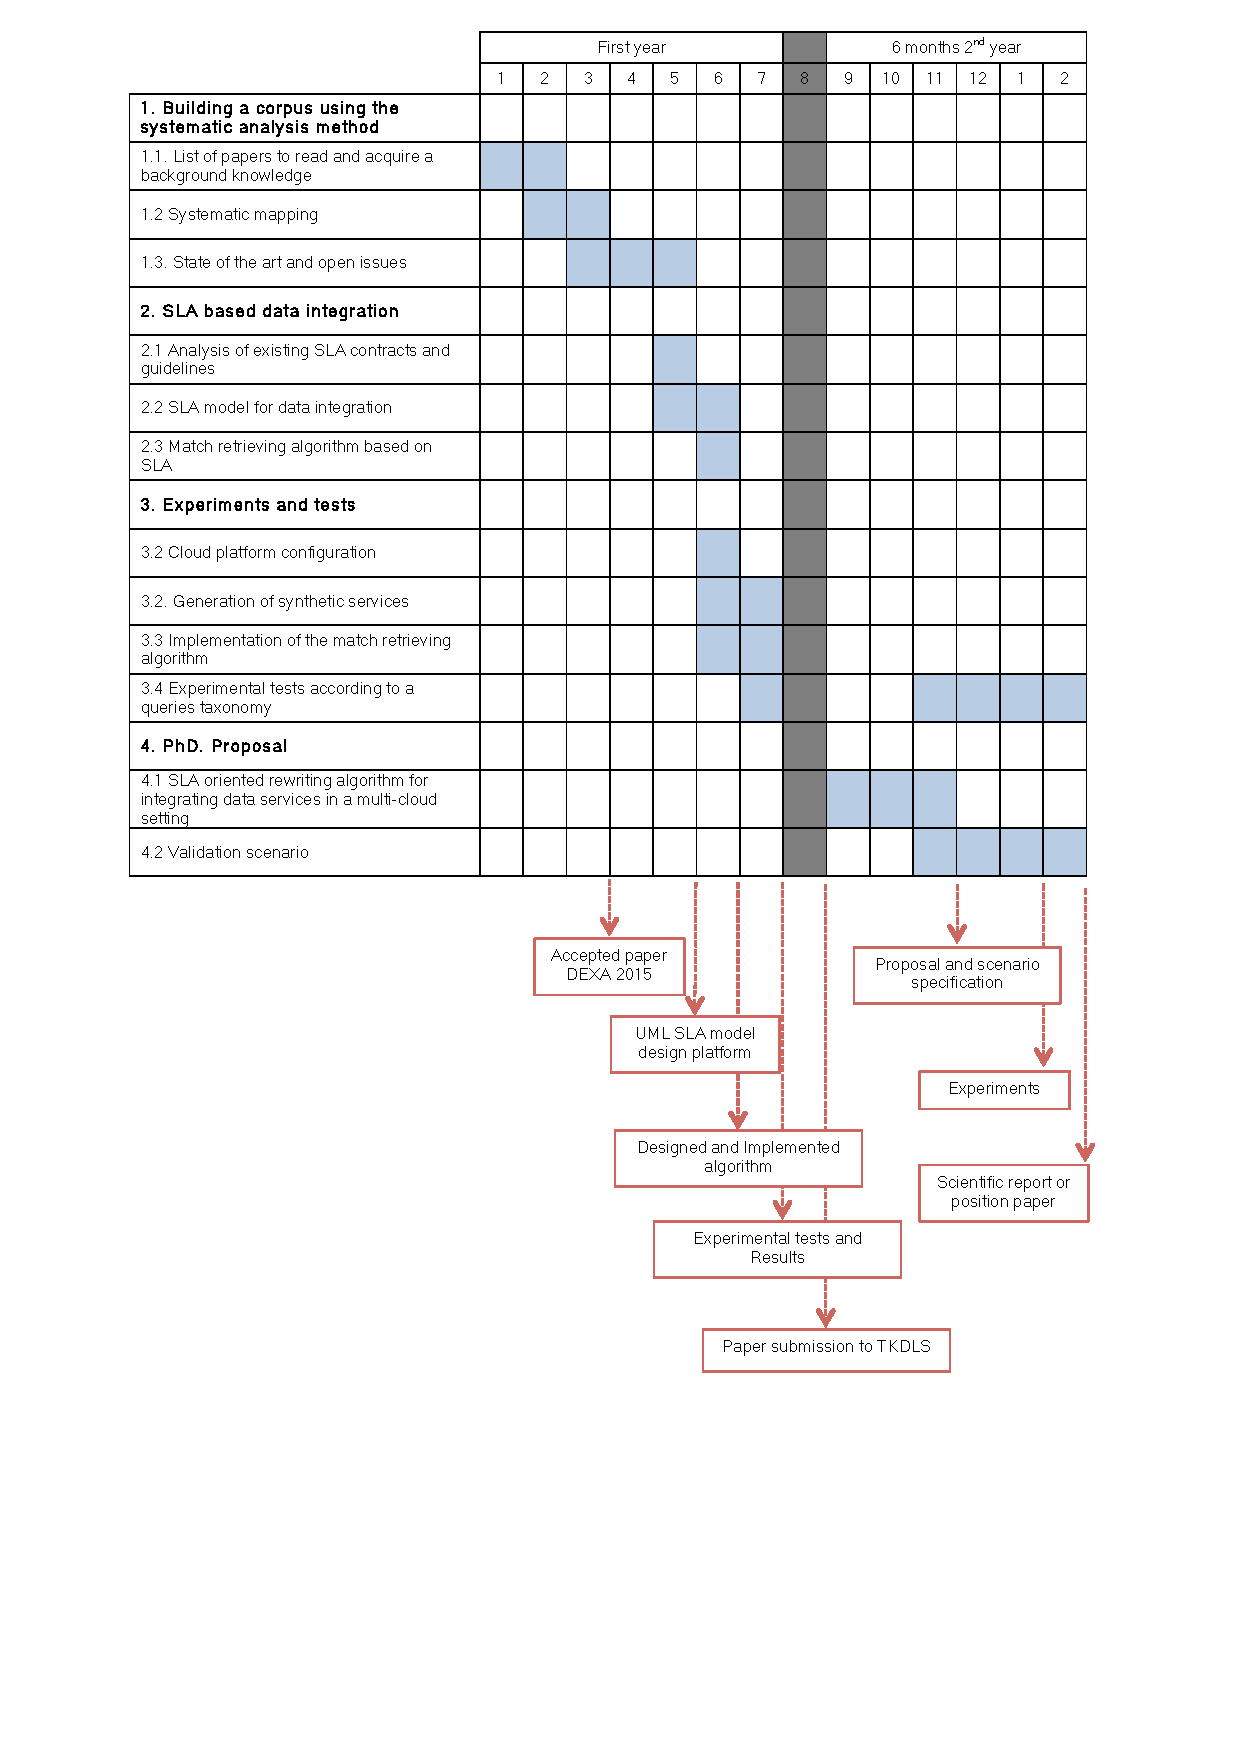
\includegraphics[scale=0.65]{calendario.png} \label{fig:calendar} \caption{Calendar}

\end{figure}

\bibliographystyle{plain}
\bibliography{bibliography}


\end{document}